% The strategist (the archivist) through one match against the yardstick: which role it
% held on each tick. Data: `lab roles archivist yardstick 0` (crates/lab), seed 0, the
% archivist in seat 0. Standalone: compiles on its own in Overleaf with pdflatex.
\documentclass[tikz,border=4pt]{standalone}
\usetikzlibrary{arrows.meta,shapes.geometric,positioning,calc}

% --- Colors: the deck's palette --------------------------------------------
\definecolor{ink}{HTML}{1B2430}     % text and axes
\definecolor{muted}{HTML}{6B7680}   % grid, notes
\definecolor{rule}{HTML}{C9CFD3}    % lane lines
\definecolor{approach}{HTML}{2F4BA0}
\definecolor{evade}{HTML}{8B2E2E}
\definecolor{stand}{HTML}{6B7680}
\definecolor{engage}{HTML}{2A6B4A}

% --- Scale: x in ticks, y in lanes --------------------------------------------
\newcommand{\Ticks}{513}    % the match's length in ticks (it ended on the last round)
\newcommand{\TickW}{0.046}  % cm per tick
\newcommand{\LaneH}{1.1}    % cm per lane
\newcommand{\BarH}{0.7}     % cm, height of a run within its lane

\begin{document}
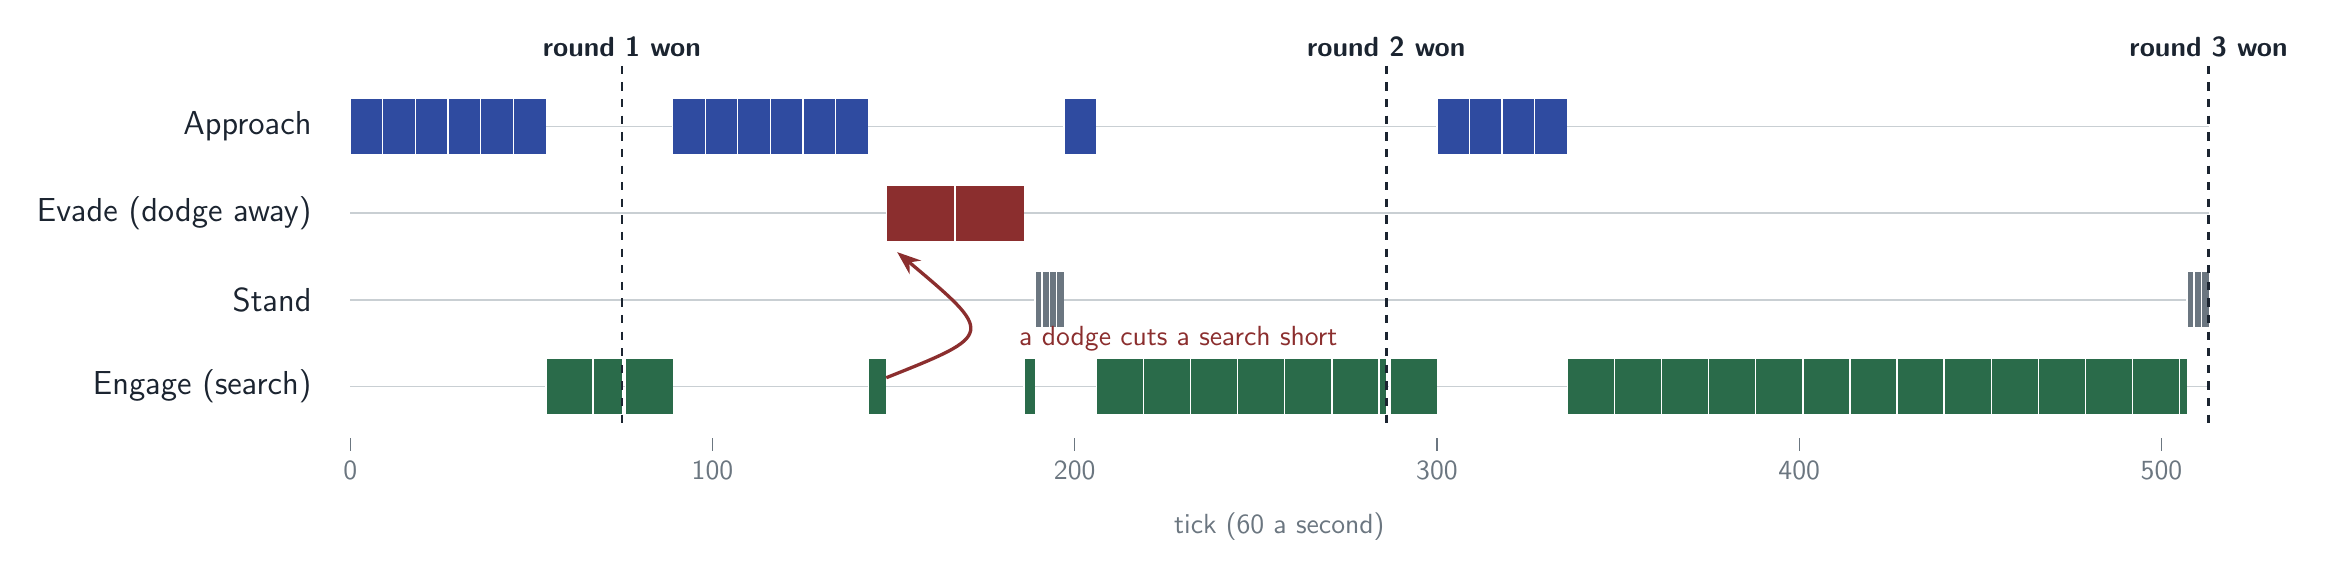
\begin{tikzpicture}[x=\TickW cm, y=\LaneH cm, font=\sffamily\large, ink]

% --- Lanes: one per role, top to bottom ---------------------------------------
\foreach \lane/\name in {0/Approach, 1/Evade (dodge away), 2/Stand, 3/Engage (search)} {
  \draw[rule, line width=0.6pt] (0, -\lane) -- (\Ticks, -\lane);
  \node[anchor=east, font=\sffamily\large] at (-8, -\lane) {\name};
}

% --- Ticks along the bottom ------------------------------------------------------
\foreach \t in {0, 100, ..., 500} {
  \draw[muted] (\t, -3.6) -- (\t, -3.75);
  \node[anchor=north, text=muted, font=\sffamily\normalsize] at (\t, -3.75) {\t};
}
\node[anchor=north, text=muted, font=\sffamily\normalsize] at (\Ticks/2, -4.35) {tick (60 a second)};

% --- Runs: each move it chose, from its first tick to its last ---------------------
\foreach \a/\b/\lane in {0/9/0, 9/18/0, 18/27/0, 27/36/0, 36/45/0, 45/54/0, 54/67/3, 67/75/3, 76/89/3, 89/98/0, 98/107/0, 107/116/0, 116/125/0, 125/134/0, 134/143/0, 143/148/3, 148/167/1, 167/186/1, 186/189/3, 189/191/2, 191/193/2, 193/195/2, 195/197/2, 197/206/0, 206/219/3, 219/232/3, 232/245/3, 245/258/3, 258/271/3, 271/284/3, 284/286/3, 287/300/3, 300/309/0, 309/318/0, 318/327/0, 327/336/0, 336/349/3, 349/362/3, 362/375/3, 375/388/3, 388/401/3, 401/414/3, 414/427/3, 427/440/3, 440/453/3, 453/466/3, 466/479/3, 479/492/3, 492/505/3, 505/507/3, 507/509/2, 509/511/2, 511/513/2} {
  \ifcase\lane \def\c{approach}\or \def\c{evade}\or \def\c{stand}\or \def\c{engage}\fi
  \fill[\c] (\a, -\lane - \BarH/2/\LaneH*1) rectangle (\b, -\lane + \BarH/2/\LaneH*1);
  \draw[white, line width=0.5pt] (\a, -\lane - \BarH/2/\LaneH*1) -- (\a, -\lane + \BarH/2/\LaneH*1);
}

% --- Round ends ------------------------------------------------------------------------
\foreach \t/\label in {75/{round 1}, 286/{round 2}, 513/{round 3}} {
  \draw[ink, line width=1pt, dashed] (\t, 0.7) -- (\t, -3.5);
  \node[anchor=south, font=\sffamily\normalsize\bfseries] at (\t, 0.7) {\label{} won};
}

% --- An interrupt ---------------------------------------------------------------------
\foreach \t in {148} {
  \draw[-{Stealth[length=3mm]}, evade, line width=1.2pt] (\t, -2.9) .. controls (\t+30, -2.4) .. (\t+3, -1.45);
  \node[anchor=west, text=evade, font=\sffamily\normalsize] at (\t+34, -2.45) {a dodge cuts a search short};
}

\end{tikzpicture}
\end{document}

% --- Self-check ----------------------------------------------------------------
% Runs: the \foreach list is `lab roles archivist yardstick 0`, each move's first and last
%   tick; the one-tick gaps between moves (the tick it chooses again) belong to the run before.
% Lanes: approach, dodge_away, stand, search, in the order of the archivist's rules.
% Round ends: the ticks of the RoundEnd events in the same trace (75, 286, 513).
% Interrupt: the first search that ended before its 12 ticks with a dodge or stand next.
